%% -----------------------------------------------------------------
%% This file uses UTF-8 encoding
%%
%% For compilation use following command:
%% latexmk -pdf -pvc -bibtex thesis
%%
%% -----------------------------------------------------------------
%%                                     _     _      
%%      _ __  _ __ ___  __ _ _ __ ___ | |__ | | ___ 
%%     | '_ \| '__/ _ \/ _` | '_ ` _ \| '_ \| |/ _ \
%%     | |_) | | |  __/ (_| | | | | | | |_) | |  __/
%%     | .__/|_|  \___|\__,_|_| |_| |_|_.__/|_|\___|
%%     |_|                                          
%%
%% -----------------------------------------------------------------

\documentclass{kithesis}

% Additional packages
\usepackage[main=slovak,english]{babel}
% For thesis written in English just change the order of languages:
% \usepackage[main=english,slovak]{babel}

\usepackage{listings}  % for source code
% Listings settings
% See for details: https://en.wikibooks.org/wiki/LaTeX/Source_Code_Listings
\lstset{
    basicstyle=\small\ttfamily,  % smaller typewriter font
    showstringspaces=false       % don't show spaces in string
}

% Location of file with bibliography resources
\addbibresource{chapters/bibliography.bib}

% Variables
%\thesisspec{figures/thesisspec.png} 

\title{My thesis \br (the skeleton)}{Využitie online AI nástrojov pri preklade programovacích jazykov}

\author[Bc.]{Július}{Sládek}[]
\supervisor{doc. Ing. Csaba Szabó PhD.} %veduci prace
%\consultant{Donald E. Knuth} %konzultant
%\college{University of Žilina}{Žilinská univerzita} %univerzita
%\faculty{Faculty of Electrical Engineering and informatics}{Fakulta elektrotechniky a informatiky} %fakulta
%\department{Department of Computers and Informatics}{Katedra počítačov a informatiky} %katedra
%\departmentacr{DCI}{KPI} % skratka katedry
\thesis{Master thesis}{Diplomová práca} %typ prace
\submissiondate{28}{01}{2024}
%\fieldofstudy{9.2.1 Informatika}
%\studyprogramme{Informatika}
%\city{Košice} %mesto
\keywords{Artificial inteligence, AI, online AI tools, programming languages, translation of programming languages}
{Umelá inteligencia, AI, online AI nástroje, programovacie jazyky, preklad programovacích jazykov}
%\declaration{som nepodvadzal}

\abstract{%
    % english 
	The thesis deals with the possibilities of using online AI tools to translate programming languages. The aim of this thesis is to investigate and verify whether these tools can be used in translation between programming languages. The thesis will explain in general terms what artificial intelligence - AI - is, its basic characteristics and division. Online tools that use artificial intelligence will also be reviewed, with increased attention to those that support working with programming languages. The selected programming languages will be briefly described and their main features and characteristics will be analysed. Experiments will be conducted where various metrics will be verified, such as translation accuracy, code efficiency, and translatability. Based on the results of the experiments, the practical use of these online AI tools in the translation of programming languages will be evaluated.
}{%
    % slovak 
	Diplomová práca sa zaoberá možnosťami využitia online nástrojov AI na preklad programovacích jazykov. Cieľom tejto práce je preskúmať a overiť či je možné tieto nástroje použiť pri preklade medzi programovacími jazykmi. V diplomovej práci bude vo všeobecnosti vysvetlené, čo je to umelá inteligencia - AI, jej základné vlastnosti a rozdelenie. Preskúmané budú aj online nástroje, ktoré využívajú umelú inteligenciu, zvýšená pozornosť sa bude venovať tým ktoré podporujú prácu s programovacími jazykmi. Vybrané programovacie jazyky budú stručne popísané a budú analyzované ich hlavné črty a vlastnosti. Vykonajú sa experimenty, kde bude overené rôzne metriky, ako napríklad presnosť prekladu, efektivita kódu, možnosť prekladu.  Na základe výsledkov experimentov sa vyhodnotí praktické využitie týchto online nástrojov AI pri preklade programovacích jazykov.
}

\acknowledgment{Na tomto mieste by som rád poďakoval svojmu vedúcemu práce doc. Ing. Csaba Szabó PhD. za dôležité rady a odborné vedenie počas riešenia mojej záverečnej práce.

Rovnako by som sa rád poďakoval svojim rodičom a priateľom za ich podporu a povzbudzovanie počas celého môjho štúdia.
}

% if you want to work only on selected chapters
%\includeonly{chapters/analyza} %,chapters/synteza}

% Load acronyms
% Acronyms
% ========
%
% An acronym is a word formed from the initial letters in a phrase. 
%
% Acronym Definition Exapmle:
% ---------------------------
% \newacronym{gcd}{GCD}{Greatest Common Divisor}
% \newacronym{dry}{DRY}{Don't Repeat Yourself}
%
% Usage:
% ------
% You can use these three options:
% 
% \acrlong{}  
%   Displays the phrase which the acronyms stands for. Put the label of the acronym inside the braces. In the example, \acrlong{gcd} prints Greatest Common Divisor. 
%
% \acrshort{} 
%   Prints the acronym whose label is passed as parameter. For instance, \acrshort{gcd} renders as GCD. 
%
% \acrfull{ } 
%   Prints both, the acronym and its definition. In the example the output of \acrfull{dry} is Don't Repeat Yourself (DRY). 
% 
% For more information see:
% -------------------------
% * https://www.sharelatex.com/learn/Glossaries 
% * https://en.wikibooks.org/wiki/LaTeX/Glossary
%


\newacronym{gcd}{GCD}{Greatest Common Divisor}
\newacronym{lcm}{LCM}{Least Common Multiple}



%% -----------------------------------------------------------------
%%          _                                       _   
%%       __| | ___   ___ _   _ _ __ ___   ___ _ __ | |_ 
%%      / _` |/ _ \ / __| | | | '_ ` _ \ / _ \ '_ \| __|
%%     | (_| | (_) | (__| |_| | | | | | |  __/ | | | |_ 
%%      \__,_|\___/ \___|\__,_|_| |_| |_|\___|_| |_|\__|
%%                                                      
%% -----------------------------------------------------------------

\begin{document}
%% Title page, abstract, declaration etc.:
\frontmatter{}

%% List of code listings, if you are using package minted
%\listoflistings

%\pagenumbering{arabic}

%% Chapters
% !TEX root = ../thesis.tex

\chaptermark{Úvod}
\phantomsection
\addcontentsline{toc}{chapter}{Úvod}

\chapter*{Úvod}

Napriek tomu že umelá inteligencia získala v posledných rokoch veľkú popularitu, tak sa nejedná o žiaden nový pojem. O umelej inteligencií sa písalo už v roku 1950. Vďaka technologickému pokroku však v posledných rokoch zaznamenala najväčší pokrok. A budúcnosť umelej inteligencie môže byť viac než pozoruhodná. 
\par Na základe veľkého pokroku v umelej inteligencii, vieme, že umelá inteligencia dokáže napodobniť ľudské činnosti. Už dnes môžeme povedať že umelá inteligencia dokáže prakticky vnímať, plánovať, riešiť problémy, myslieť, rozumieť, učiť sa. Tieto vlastnosti umelej inteligencie sú základným pilierom pre jej ďalší vývoj smerom k budúcnosti.
\par Umelá inteligencia a digitálna transformácia sú dotýkajú vo väčšej miere dokonca našich moderných životov. Toto zrýchlené tempo v súčasnej dobe poháňa umelú inteligenciu na vyššiu úroveň. Už dnes máme dostatočné množstvo AI online nástrojov, ktoré nám uľahčujú nielen každodenný život ale i programovanie.
 Umelá inteligencia otvára nové možnosti a zrýchluje pokrok v širokom spektre odvetví.
\par V diplomovej práci sa zameriavame na teoretické poznatky o umelej inteligencii, jej štruktúre, AI online nástrojoch, ich úlohe v programovaní, prekladu programovacích jazykov a pohľadu do budúcnosti umelej inteligencii. 
\par V druhej časti diplomovej práce zanalyzujeme dostupné online AI nástroje a preskúmame potenciál AI online nástrojov na použitie pri preklade programovacích jazykov. V analytickej časti diplomovej práci sa zameriavame najmä na faktory akými sú presnosť prekladu, podpora programovacích jazykov, dopad na výkon a riešenie prekladu špecifických jazykových konštrukcií, ktoré iné jazyky priamo nepodporujú. V analytickej časti vytvoríme vlastné experimenty, čím sme schopní vyhodnotiť využitie AI online nástrojov pri preklade programovacích jazykov.

Uvod sa ešte pozmení a doplní keď bude hotová celá DP



\section*{Formulácia úlohy}
Cieľom diplomovej práce je analyzovať dostupné AI online nástroje a preskúmanie ich potenciálu na použitie pri preklade programovacích jazykov. Je potrebné zamerať sa na hlavné faktory ktorými sú:
\begin{itemize}
\item presnosť prekladu
\item podpora programovacích jazykov
\item efektivita kódu
\item riešenie prekladu špecifických jazykových konštrukcií, ktoré iné jazyky priamo nepodporujú
\end{itemize}

Po oboznámení sa zo zadaním úlohy sme vyhodnotili že riešenie bude nasledovné:
\begin{itemize}
\item Vo všeobecnosti sa oboznámime s pojmom umelá inteligencia (AI) a zistíme aké má využitie, prínosy a delenie
\item Oboznámime sa s AI online nástrojmi a preskúmame aké nástroje sú dostupné na riešenie nášho problému
\item Preskúmame programovacie a vyberieme jazyky, ktoré budú využité pri experimentoch
\item Vytvoríme experimenty, kde otestujeme všetky požadované parametre 
\item Na záver zanalyzujeme výsledky experimentov, vyvodíme závery a zhodnotíme praktické využitie  prekladu programovacích jazykov pomocou online AI nástrojov. 
\end{itemize}


% !TEX root = ../thesis.tex

\chapter{Analýza umelej inteligencie}

Súčasný stav riešenej problematiky doma i v zahraničí rieši teoretické poznatky v oblasti AI a úloh AI online nástrojov v programovaní.  Dôvodom spracovania teoretických poznatkov o AI, čo je základ pre tvorbu analytickej časti, je práve AI, ktorá sa stáva viac výkonnejšou so všestranným použitím. Za týmto úspechom stojí práve rozvoj výpočtového výkonu, prístup k obrovským údajom alebo pokrok v algoritmoch, na základe ktorých je postavená AI.
\par Je dôležité sa pozrieť na AI, ktorá formuje trh nielen na regionálnej ale i globálnej úrovni, v súčasnosti poznačenou digitálnou transformáciou a neustále meniacim sa technologickým prostredím. 



% ------------------- Definícia Artificial Intelligence (AI) z pohľadu literatúry -------------------------


\section{Definícia Artificial Intelligence (AI) z pohľadu literatúry}

Artificial Intelligence (ďalej skr. AI) znamená v preklade umelá inteligencia. Umelá inteligencia má mnoho definícií. AI ako spojenie dvoch slov „umelá“ a „inteligencia“ možno chápať ako stroje, ktoré dokážu simulovať inteligenciu. \cite{1article} Aby sme mali schopnosť vystihnúť zmysel umelej inteligencie, je nevyhnutné pozrieť sa aj na iné definície od rôznych autorov z blízkej minulosti.
\par V roku 2017 Kolbjørnsrud et al. definoval AI ako počítače a aplikácie, ktoré vnímajú, chápu, konajú a učia. \cite{2article} V roku 2019 Afiouni definoval AI ako všeobecný koncept pre počítačové systémy schopné vykonávať úlohy, ktoré zvyčajne vyžadujú prirodzenú ľudskú inteligenciu. \cite{3conference} V tom istom roku  Lee et al. konkrétnejšie zadefinoval AI ako inteligentné systémy, ktoré sú určené na používanie údajov, spracovanie analýz a sústreďujú pozornosť na automatické vykonávanie úloh bez toho, aby boli tieto inteligentné systémy naprogramované.\cite{4article} Wang et al. (2019) len vo všeobecnosti zhrnul AI ako inteligentný stroj, pretože podľa neho AI je dosť široký pojem. Už Makarius (2020) bližšie špecifikoval AI ako niečo dosť inteligentné, čo je schopné zanalyzovať údaje tak, aby bolo možné z toho vyťažiť dôležité informácie nevyhnutné na dosahovanie cieľov s prvkom flexibility. Schmidt et al. (2020) v porovnaní s Makariusom v danom roku definoval AI ako snahu napodobniť kognitívne a ľudské schopnosti na počítačoch. \cite{5article} Autori ako Demlehner a Laumer (2020) definovali AI ako inteligentný systém, ktorý nielen vníma, chápe, učí alebo posudzuje, ako tvrdil Kolbjørnsrud v roku 2017, ale ako systém, ktorý dokáže plánovať explicitne bez vopred naprogramovania, vopred zadaných pravidiel a akcií, rovnako poznamenal Lee et al. v roku 2019. Autor Wamba-Taguimdje et al. (2020) definoval AI ako teórií a techník, ktoré sa používajú na vývoj takých strojov, ktoré simulujú inteligenciu bez toho, aby tieto stroje (počítače) boli použité na modelovanie inteligentného správania sa bez zásahu ľudskej bytosti. Autori Mikalef a Grupta (2021) definovali AI ako schopnosť systému zanalyzovať, interpretovať a zhrnúť dôležité výstupy zo zbieraných dát. Kanade (2022) tvrdí, že AI ako systém v zásade vnímajú prostredie, rozpoznávajú objekty, prispievajú k rozhodovaniu, riešia zložité problémy, učia sa z minulých skúseností a napodobňujú vzory. \cite{6article}AI predstavuje technológie ako je strojové učenie, spracovanie prirodzeného jazyka, počítačové videnie a ďalšie. Kanade (2022) poukázal prostredníctvom týchto definícii na to, že tieto špičkové technológie a ich inteligentné systémy porozumejú ľudskej reči a dokonca dokážu prognózovať. Dnes pojem AI popisuje širokú škálu technológií, ktoré poháňajú mnohé služby a produkty, ktoré používame každý deň - od aplikácií až po chatbotov. \cite{7article}
\par Z pohľadu histórie o definíciách AI je zrejmé, že všetky činnosti kedysi vykonávala ľudská bytosť a v súčasnosti AI napodobňuje ľudské činnosti. Ale vzniká tu otázka do akej miery je AI v súčasnosti tak schopná napodobniť ľudskú inteligenciu a rozumieť ľudskému prirodzenému jazyku.


% ---------------------------- Evolúcia AI - vývoj a technologické výzvy ----------------------------------


\subsection{Evolúcia AI - vývoj a technologické výzvy}

Vývoj AI a nezodpovedané otázky v oblasti počítačovej vedy sa začali riešiť ešte v roku 1956 pri prítomnosti významných vedcov ako napríklad John McCarthy, Marvin Minsky, Natahniel Rochester, Claude Shannon a ďaľší,  Po tomto stretnutí začala prvá AI „jar“, ktorú však brzdili vtedajšie hardvérové a softvérové podmienky. \cite{tencent2021}
\par Vývoj AI prebiehal takmer šesťdesiat rokov. Najväčšia explózia s AI nastala približne pred šiestimi rokmi. Aj štatistické prieskumy dokazujú rastúcu tendenciu v počte podnikov využívajúcich AI ale i rastúcu tendenciu investovania do AI. V nasledujúcom grafe na obrázku č. 1.1 si znázornime aký priebeh vo vývoji nastal AI z pohľadu histórie. 

\begin{figure}[!ht]
    \centering
    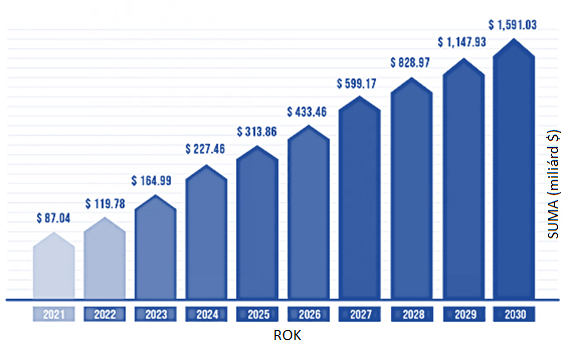
\includegraphics[width=1\textwidth]{figures/graf1.png}
    \caption{Graf s velkosť trhu s AI\label{Graf s velkosť trhu s AI}}
\end{figure}

Graf na obrázku č. 1.1  nepoukazuje len na ohromujúci vývoj AI ale i vplyv AI na podniky, ekonomiku a náš každodenný život. Trh AI v roku 2030 bude predstavovať až 1 591 03 miliard dolárov. Táto prognóza hovorí až o 18\% náraste za deväť rokov (2021-2030). 
\par Robotika a spracovanie prirodzeného jazyka až po etické otázky vo vývoji AI predstavujú pokročilé technológie. \cite{toolsforhumans2023} Dnešní ľudia spustili skutočne inteligentnú revolúciu, čo je spôsobené technologickými objavmi a masovým šírením AI. 
\par Dvadsiate prvé storočie je obdobím veľkým zmien v AI. Aj príchod hlbokého učenia (deep learning alebo inak povedané strojové učenie) spustil v AI prudký nárast.  To znamená, že ide o pokročilú technológiu alebo vyšší stupeň AI inšpirovaný ľudskou inteligenciou. AI dokáže v súčasnosti porozumieť obsahu obrázka, videa, komunikovať medzi ľuďmi písomnou formou alebo prostredníctvom jazyka, dokáže vytvoriť zásobáreň informácií, ktoré sa neustále zdokonaľujú, riadia autá a podobne.  Ide o medzidisciplinárnu vedu, ktorá pokrýva mnoho oblastí vrátane informatiky, štatistiky, neurológie a spoločenských vied. \cite{tencent2021}
\par V oblasti spracovania prirodzeného jazyka existuje veľa techník a metód, ako dosiahnuť priaznivé výsledky.  V roku 2017 sa však objavila technológia, ktorá predčila všetky doposiaľ aplikované pokusy o vytvorenie dokonalého generátora človekom-písaného textu.  Transformery sa začali používať na modelovanie neurónových sietí od ich vzniku a priniesli mnohé dych-berúce modely. \cite{novotny2020}
\par Budúci vývoj AI smeruje k rýchlostnej, kvalitatívnu a kolektívnu superinteligenciu s prvkami toho, čo prekonáva ľudskú bytosť a hlavne z pohľadu rýchlosti spracovávania informácií, väčšieho výkonu, kvality, schopnosti riešenia problému alebo využívania plného potenciálu AI v budúcnosti, konštatuje Vrba (2019, s. 17).
\par Z pohľadu evolúcie AI a rozmachu pokročilých technológií možno tvrdiť, že prínos AI bude značný, ak sa odstránia niektoré jej slabiny. No vyžaduje si to neustále napredovanie v tomto technickom a digitálnom svete, kedy rýchlosť, kvalita, výkon sú základnými faktormi pre efektívne využitie plného potenciálu AI. Toto možno považovať za evolúciu, kde tempo, rýchlosť a objem dát je už neudržateľný a vymyká sa to už ľudským schopnostiam. \cite{hlasny2023} A preto je nevyhnutné si uvedomiť aké dôležité sú pokročilé technológie a AI. Umelá inteligencia je tvorená ľuďmi a jej smerovanie bude závisieť aj od kolektívneho vedomia ľudí. Umelá inteligencia nepochybne časom otvorí nový svet. \cite{tencent2021}



% -------------------------------------- Elementárne vlastnosti AI ---------------------------------------

\subsection{Elementárne vlastnosti AI}

AI a jej aplikácia je využiteľná v rôznych oblastiach. Podľa prognózy (graf na obrázku č. 1.1) trh AI rastie, čo odráža aj fakt, že rastie priamo úmerne aj počet podnikov implementujúce AI do svojej praxe. Avšak niektoré odvetvia viac aplikujú AI a v iných odvetviach je aplikácia AI ešte na slabšej úrovni. Na nasledujúcom obrázku č. 1.2 si znázorníme ako umelá inteligencia mení jednotlivé odvetvia.

\begin{figure}[!ht]
    \centering
    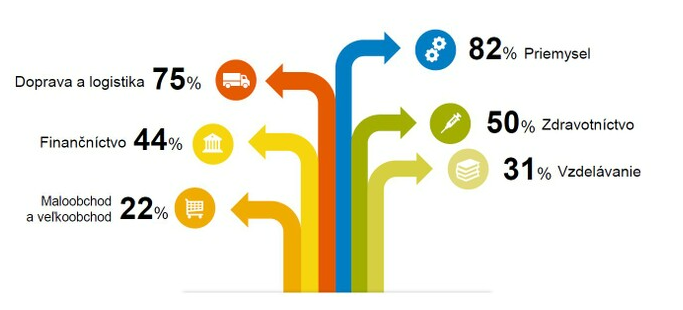
\includegraphics[width=1\textwidth]{figures/AI-a-jej-aplikacia-v-odvetviach.png}
    \caption{AI a jej aplikácia v odvetviach}
\end{figure}

Na obrázku č. 1.2 môžeme vidieť, že uplatnenie AI je najvýraznejšie v priemysle (82 \%), doprave a logistike (75 \%). Aby technológie AI nachádzali široké uplatnenie aj v ostatných priemysloch je nevyhnutná znalosť vlastností AI.
Preto v nasledujúcej tabuľke č. 1 zhromaždíme elementárne vlastnosti AI.



\begin{table}[!ht]
    \centering
    \begin{tabular}{|p{2.5cm}|p{2.5cm}|p{2.5cm}|p{2.5cm}|p{2.5cm}|}
    \hline
       \multicolumn{5}{|c|}{Názvy} \\ \hline
        Konanie ľudsky & Myslenie ľudsky & Myslenie rozumne & Konanie rozumne & Učenie   \\ \hline
        Plánovanie  & Rozpozn. reči & Riešenie problému & Vedomosti  & Vnímanie   \\ \hline
    \end{tabular}
    \caption{\label{table1}Vlastnosti AI}
\end{table}

\par \textbf{Konanie ľudsky:}  Autor Kurzweil (1990) to chápal ako umenie vytvárať stroje, ktoré vykonávajú funkcie, ktoré vyžadujú inteligenciu, keď ich vykonávajú ľudia. \cite{ayca2019} Iná definícia chápe túto vlastnosť ako štúdiu o tom, ako prinútiť počítače robiť veci, v ktorých sú ľudia v súčasnosti lepší. \cite{ayca2019} Ide o vlastnosť AI systémov, ktoré napodobňujú ľudské správanie sa ako napríklad aj porozumenie prirodzeného jazyka. Táto vlastnosť AI je vyvíjaná do takej miery, aby sme nerozoznali AI od ľudskej bytosti. 
 \\
\par \textbf{Myslenie ľudsky:} Haugeland (1985) chápal túto vlastnosť ako vzrušujúce nové úsilie prinútiť počítače myslieť...stroje s mysľou v plnom a doslovnom zmysle. \cite{ayca2019} Predchodca Bellman (1978) chápal túto vlastnosť ako automatizácia činností s ľudským napodobňuje ľudské myslenie a kognitívne funkcie. Ide o vlastnosť AI, ktorej cieľom dosiahnuť kognitívnu podobnosť s ľudským myslení.
 \\
\par \textbf{Konanie racionálne:} Nilson (1998) chápal túto vlastnosť AI ako inteligentné správania sa. \cite{ayca2019} Táto vlastnosť AI v porovnaní s konaním ľudsky je odlišná v tom, že konanie ľudsky sa zameriava na napodobňovanie ľudského správania sa a konanie racionálne kladie dôraz na prijímanie takých rozhodnutí, ktoré sú v súlade s logickým uvažovaním pre dosiahnutie cieľov.
 \\
\par \textbf{Myslenie racionálne:} Charniak a McDermott (1985) chápali túto vlastnosť ako štúdium mentálnych schopností pomocou výpočtových modelov. \cite{ayca2019} Winston (1992) chápal túto vlastnosť ako štúdium výpočtov, ktoré umožňujú vnímať, uvažovať a konať. \cite{ayca2019} Myslenie racionálne je vlastnosťou AI systémov, ktoré sa rozhodujú na základe logického uvažovanie a racionálneho rozhodovania, ktoré vedú k optimálnym výsledkov pre dosiahnutie cieľov.
 \\
\par \textbf{Učenie:} Táto vlastnosť je dôležitá v tom, aby systémy AI sa dokázali adaptovať, zlepšovať svoje rozhodovacie procesy pri plánovaní a hlavne aby dokázali efektívnejšie vykonávať úlohu, ak pribudnú nejaké nové informácie alebo situácie. Touto schopnosťou sa AI systémy učia zlepšovať svoj výkon.
 \\
\par \textbf{Plánovanie:} AI dokáže formulovať stratégie a pripraviť plány dôležité pre dosiahnutie konkrétnych cieľov, ktoré preukazujú úroveň predvídateľnosti pri strategickom rozhodovaní. Plánovanie v AI funguje na základe algoritmov a rozhodovacích výpočtových procesov. Plánovanie v AI dokáže formulovať stratégie a plány aj v tých zložitých a dynamických prostrediach.
 \\
\par \textbf{Rozpoznávanie reči:} Táto vlastnosť AI systémov je odlišná od iných vlastností v tom, že sa snaží nielen porozumieť ľudskej bytosti ale i interpretovať. Technológia rozpoznávania reči využíva algoritmy a techniky strojového učenia na analýzu zvukových signálov a presný prepis hovorového slova. Touto vlastnosťou AI je vyvíjaná snaha o interakciu ľudskej bytosti s počítačom. Takže ľudská bytosť dokáže komunikovať so systémami AI prostredníctvom prirodzeného hovoreného jazyka.
 \\
\par \textbf{Riešenie problémov:} AI dokáže riešiť problémy, analyzovať a generovať informácie, ktoré nám poskytnú vhodné riešenie.
 \\
\par \textbf{Vedomosti:} Spracovanie znalostných vedomostí je v súčasnosti dominantnou paradigmou inteligentných technológií. Systémy, ktoré sa zvyčajne označujú ako „inteligentné“, sú systémy, ktorých dominantným základom je znalostná báza alebo doménový model popísaný jazykom na vysokej úrovni, takmer prirodzený. \cite{kornienko2015}
 \\
\par \textbf{Vnímanie:} AI dokáže vnímať prostredie a interpretovať prostredníctvom rôznych inteligentných zariadení simulujúce ľudské vnímanie ako napríklad kamery, senzory a iné. 
Keďže AI sa stáva pre organizácie čoraz dôležitejším aktívom, tvrdí Enholm et al. (2021) \cite{enholm2022}, by mali podniky vedieť implementovať také aplikácie pre podporu svojich činností na základe poznania vlastností, ktoré AI ponúka.  \cite{article} 

\par Dôležitým poznatkom v oblasti AI je nielen ohromujúca snaha o napodobenie ľudského myslenia a ľudského správania sa ale i to, ako kooperáciou týchto vlastností AI dokáže dospieť k pozoruhodným výstupom. Vieme, že vlastnosti AI systémov sú zdokonaľované postupne a v súčasnosti už pozorujeme ich značnú úroveň.


% -------------------------------------- Štruktúra AI systémov -------------------------------------


\subsection{Štruktúra AI systémov}

Každý informačný systém sa skladá z niekoľkých komponentov, ktoré sú dôležité pre dosiahnutie efektivity a inovácií v oblasti AI. AI systém možno rozdeliť do šiestich stavebných blokov ako môžeme vidieť na obrázku č. 1.3

\begin{figure}[!ht]
    \centering
    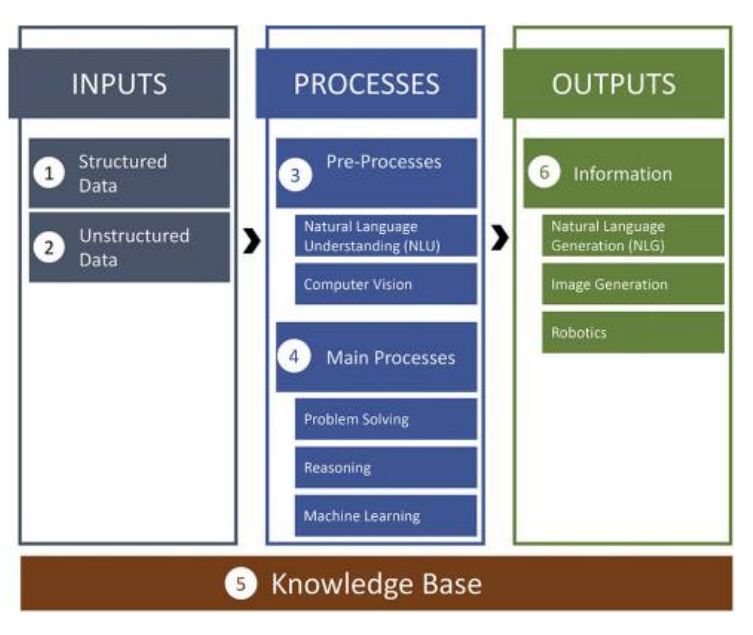
\includegraphics[width=1\textwidth]{figures/stavebne-bloky-ai-systemov.png}
    \caption{Stavebné bloky AI systémov}
    \end{figure}

Podľa obrázka č. 1.3 je zrejmé, že AI systémy sa skladajú zo vstupov pozostávajúcich zo štruktúrovaných a neštruktúrovaných dát, z činností predchádzajúcich hlavným procesom a to spracovania prirodzeného jazyka NLP a počítačového videnia, z hlavných procesov ako riešenie problémov, strojové učenie, uvažovanie. Poslednými prvkami AI systémov sú databázové úložisko (databáza znalostí) a výstupy pozostávajúce z informácií získaných z generovania prirodzeného jazyka, generovania obrazu a robotiky. \cite{paschen2020}

\par \textbf{Štruktúrované dáta:} Štruktúrované dáta sú štandardizované a usporiadané dáta, ktoré tvoria jadro analýzy.  Príkladom štruktúrovaných dát sú dáta napríklad o zásobách podniku, o predajoch a iné. AI systém ich dokáže analyzovať v reálnom čase. \cite{paschen2020}
\\
\par \textbf{Neštruktúrované dáta:} Neštruktúrované dáta na rozdiel od štruktúrovaných dát sa vyznačujú zložitosťou ich analyzovania. AI systém ich dokáže zanalyzovať tieto dáta, aby nám poskytli dôležitú informáciu. 
\\
\par \textbf{Činnosti pred hlavnými procesmi:} Porozumenie prirodzeného jazyka NLP a počítačové videnie sú činnosťami, ktorými sa neštruktúrované dáta vyčistia, transformujú a vyberú dáta pre ďalšie spracovanie. \cite{paschen2020}
\\
\par \textbf{Hlavné procesy:} Hlavné procesy v AI zahŕňajú 3 typy inteligentného správania: riešenie problémov, uvažovanie a strojové učenie. \cite{paschen2020}
\\
\par \textbf{Databázové úložisko znalostí:} Inteligentné správanie sa spolieha na uchovávanie minulých dát, informácií alebo znalostí. Takže skúseností, ktoré sa odrážajú v týchto znalostiach, môžu ovplyvniť následné správanie. \cite{paschen2020}
\\
\par \textbf{Informácie:} Po ukončení predchádzajúcich činností alebo procesov v AI sú výstupom zmysluplné informácie, ktoré môžu byť použité na rôzne účely ako napríklad výstup pri strategickom rozhodovaní sa podnikov alebo ako vstup do iných informačných systémov. \cite{paschen2020}
\par Štruktúra AI je základným pilierom, od ktorej závisí implementovanie AI do praxe a použitie jednotlivých typov AI a výbere tých správnych algoritmov pre efektívnu správu AI systémov. 



% -------------------------------- AI a techniky (typy a alogritmy) --------------------------------------

\subsection{AI a techniky (typy a alogritmy)}

Poznáme rôzne typy AI, ktoré sú založené na rôznych algoritmov. Poznanie typov umelej inteligencie a algoritmov nám poskytuje prehľad o možnostiach a aplikácii AI technológii do našej praxe. Poznanie typov AI a algoritmov je dôležité pre úspešné navrhovanie, implementáciu a správu AI systémov v dnešnom technologickom svete.


\begin{table}[!ht]
    \centering
    \begin{tabular}{|p{4.1cm}|p{4.1cm}|p{4.1cm}|}
    \hline
       \multicolumn{3}{|c|}{Názvy} \\ \hline
        Strojové učenie (machine learnig ML) & Hlboké učenie (deep learning DL) & Spracovanie prirodz. jaz. (natural language processing NLP)    \\ \hline
        Počítačové videnie (computer vision)  & Neurónová siete (neural networks)  & Robotika (robotics)   \\ \hline
    \end{tabular}
    \caption{\label{table2}Typy AI}
\end{table}

\textbf{Strojové učenie:} Strojové učenie je typ AI s technikami, ktoré umožňujú počítačom učiť sa z údajov a zo skúsenosti. Cieľom strojového učenia je vytvárať algoritmy, ktoré analyzujú údaje. Algoritmy strojového učenia používajú výpočtové metódy na získanie informácií priamo z údajov bez toho, aby boli explicitne vopred naprogramované.  Algoritmy adaptívne zlepšujú svoj výkon so zvyšujúcim sa počtom vzoriek dostupných na učenie.  
Strojové učenie sa delí na dva typy: učenie s učiteľom a učenie bez učiteľa. Prvý model (učenie sa s učiteľom) aplikuje tzv. učenie sa od minulých vzorov prác s dátami na účely predikcie budúcich udalostí.  Druhý model (učenie sa bez učiteľa) sa aplikuje, keď údaje nemožno klasifikovať a snahou je odhaliť skryté vzťahy medzi údajmi. \cite{stalmachova}
Na nasledujúcom obrázku č. 1.4 si znázornime členenie strojového učenia a jeho algoritmy.
\\

\begin{figure}[!ht]
    \centering
    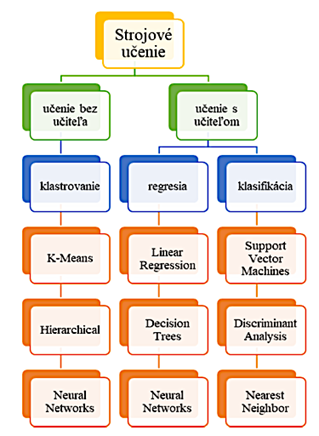
\includegraphics[width=.60\textwidth]{figures/strojove-ucenie.png}
    \caption{Strojové učenie a algoritmy}
\end{figure}

\textbf{Hlboké učenie:} Hlboké učenie je kategória strojového učenia zaoberajúca sa neurónovými sieťami s väčšou hĺbkou - mnoho neurónových vrstiev, okrem základných vstupových a výstupových vrstiev existujú skryté vrstvy. Čo znamená, že hlboké učenie umožňuje AI systémom automaticky naučiť sa prezentovať údaje v niekoľkých vrstvách. Každá vrstva v sieti vykonáva nelineárne transformácie dát, ktoré sme sieti predali ako vstupné. \cite{glos_prace_kristian}
\\

\begin{figure}[!ht]
    \centering
    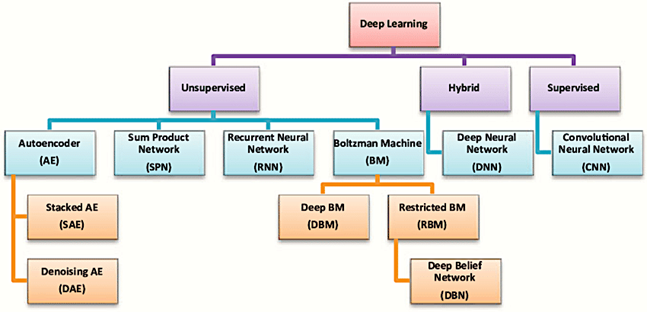
\includegraphics[width=1\textwidth]{figures/hlbkove-ucenie.png}
    \caption{Hlbkové učenie a algoritmy}
\end{figure}

\textbf{Spracovanie prirodzeného jazyka:} Spracovanie prirodzeného jazyka (NLP) je štúdium a aplikácia techník a nástrojov, ktoré umožňujú počítačom spracovávať, analyzovať, interpretovať a uvažovať o ľudskom jazyku. \cite{nelson_nlp} Medzi techniky NLP patria:

\begin{itemize}
    \item uznanie pomenovanej entity
    \item generovanie prirodzeného jazyka
    \item jednotnosť slovného významu
\end{itemize} 

Spracovanie prirodzeného jazyka používa algoritmy, ktoré sú schopné transformovať neštruktúrované údaje na štruktúrované údaje.  Je to zložitý proces, algoritmy by mali byť aplikované správnym spôsobom, aby počítač dokázal odvodiť správny význam textu.  To môžeme často spozorovať pri preklade textu medzi jazykmi.\cite{nelson_nlp}
\\
\par \textbf{Počítačové videnie:} Počítačové videnie je zložitou a špičkovou technológiou, ktorá sa opiera o AI a strojové učenie s tým rozdielom, že počítačové videnie spočíva v tom, že počítač naučia pozerať a správne interpretovať obrázky ako človek. \cite{chernyak_computer_vision} Jeho cieľom je, aby počítače vykonávali ľudské činnosti s cieľom zvýšiť efektívnosť a znížiť chybovosť. 
Počítačové videnie je metóda, ktorou počítače rozumejú a vidia digitálne obrázky a nielen ich rozpoznávajú alebo kategorizujú.  Aplikácie počítačového videnia používajú senzory a algoritmy učenia na extrahovanie komplexných informácií, ktoré sa môžu potom použiť na automatizáciu alebo informovanie iných procesov. \cite{sap_ai}
\\
\par \textbf{Neurónová sieť:} Neurónové siete sú výpočtové počítačové systémy, ktoré sú medzi sebou prepojené a ich princíp spočíva v spôsobe spracovávania informácií podobne ako v ľudskom mozgu.  Vďaka neurónovým sieťam máme možnosť klasifikovať a zhlukovať neoznačené údaje podľa podobností medzi vstupmi a označenými súbormi, pomocou ktorých sú trénované. \cite{krajci2020} Neurónová sieť je matematický model zložený z umelých neurónov a tento model je možné použiť pri rozpoznávaní obrazov, prirodzeného jazyka, rozpoznávaní hlasu a podobne. 
\\
\par\textbf{Robotika:} Robotika je nám dosť známa a v robotike boli zaznamenané veľké pokroky. Robotika je jednou z najdôležitejších oblastí priemyslu a výskumu moderného ľudstva.  Obrovským skokom vpred sa však zrejme stane technológia, ktorá otvorí úplne nové možnosti.  Tento AI systém potrebuje pre spoľahlivú funkciu kamery, z ktorej analyzuje každý pixel a vyhodnotí, z akého materiálu sú predmety vyrobené.  To si v súčasnosti vyžaduje oveľa výkonnejšiu AI, aby robot dokázal vlastnosť materiálu, rozpozná nástroj, predmet a iné. \cite{tokoly_technologia}
\par Dôležitým postrehom je ako jednotlivé typy AI a algoritmy sú navrhnuté, ako fungujú a aký technologický pokrok nastal a aké hodnoty môžu priniesť v rôznych odvetviach. Pretože tieto technológie môžu priniesť vyššiu efektivitu, automatizáciu a riešenie zložitých úloh alebo problémov. Ich význam sa v súčasnosti čoraz viac zdôrazňuje, pretože typy AI a algoritmy sú dôležitými nástrojmi pri riešení rôznych úloh.



% ------------------------------ Vyuižívanie AI a digitálna transformácia) --------------------------------

\subsection{Vyuižívanie AI a digitálna transformácia}

V súčasnosti je digitalizácia považovaná za nevyhnutnosť. Pretože implementovaním moderných digitálnych technológií sa mení spôsob akým podniky fungujú a ako môžu optimalizovať svoje procesy, aby boli efektívnejšie.
\par Kane et al. vo svojej štúdii v roku 2017 poznamenal, že procesom digitalizácie v súčasnosti ešte neprešlo mnoho podnikov (iba 25 \%).  Mnoho podnikov (41 \%) je ešte na ceste digitálnej transformácie a mála časť podnikov (34 \%) sa zatiaľ venuje len teoreticky problematike o trendoch digitálnej transformácie.  Pozoruhodným javom v jeho štúdii bol fakt, že skoro všetci manažéri podnikov (až 85 \%) boli jednoznačne za to, že digitálna zrelosť je rozhodujúcim faktorom pre úspech podnikov. \cite{holmstrom2022}
\par Rok 2020 bol prelomový v oblasti digitálnej transformácie, čo spôsobila najmä pandémia COVID-19.  Štatistiky poukazovali na rýchlejšiu digitálnu transformáciu podnikov počas pandémie v porovnaní so štatistikami za posledné desaťročie.  Adaptácia moderných digitálnych technológií nebola viac luxusom na investovanie do technológií. Adaptácia moderných digitálnych technológii sa v súčasnosti stala otázkou prežitia podnikov. \cite{aspecta_trendy_2021} Na nasledujúcom obrázku č. 1.6 sú znázornené nové výzvy digitálnej transformácie. 


\begin{figure}[!ht]
    \centering
    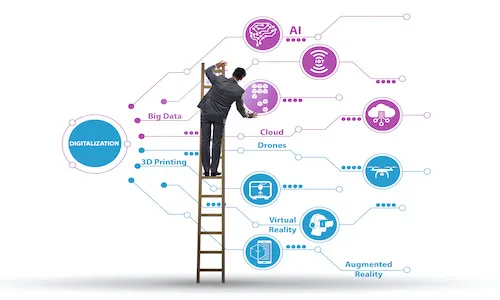
\includegraphics[width=1\textwidth]{figures/digitalna-transformacia.png}
    \caption{Digitálna transformácia}
\end{figure}

Ako môžeme vidieť na obrázku č. 1.6 medzi súčasné výzvy alebo trendy v digitálnej transformácie patria: virtuálna reality, 3D tlačiarne, drony, cloud platformy, veľké dáta a v neposlednom rade spomínaná AI. Práve AI ako nová výzva digitálnej transformácie sa stáva taktiež neoddeliteľnou súčasťou pre implementovanie do praxe podnikov.  Keďže výpočtový výkon je stále dostupnejší a cloud umožňuje prístup k tomuto výpočtovému výkonu, ako aj k softvéru a rámcom, umelú inteligenciu využíva stále viac a viac podnikov. \cite{holmstrom2022}
\par Umelá inteligencia pomáha vytvárať nástroje a riešenia, ktoré môžu automatizovať bežné úlohy, znižovať pracovné zaťaženie a súčasne zvyšovať efektivitu.  Čo sa týka rôznych inovácií v oblasti digitálnej transformácie, čo je poháňané AI, musí sa vyriešiť problematika adaptácie AI.  Nemali by podniky čakať na iný moment, pretože budúcnosť je neobmedzená a budúcnosť čaká. \cite{emea_digital_transformation_framework}
\par Dôležitým poznatkom je to, že digitálna transformácia spolu umelou inteligenciou patria medzi neoddeliteľné súčasti našich moderných životov. So zrýchleným tempom v digitálnej transformácie a v oblasti AI sa začali vyvíjať online nástroje, ktoré sú poháňané práve AI. 



% --------------------------------- Prínosy AI online nástrojov ------------------------------------

\subsection{Prínosy AI online nástrojov}

AI online nástroje nás už sprevádzajú pomaly všade. Na nasledujúcom obrázku č. 1.7 je znázornené kde AI je využívaná na každodennej báze a jej budúci potenciál, kde AI možno implementovať do praxe.

\begin{figure}[!ht]
    \centering
    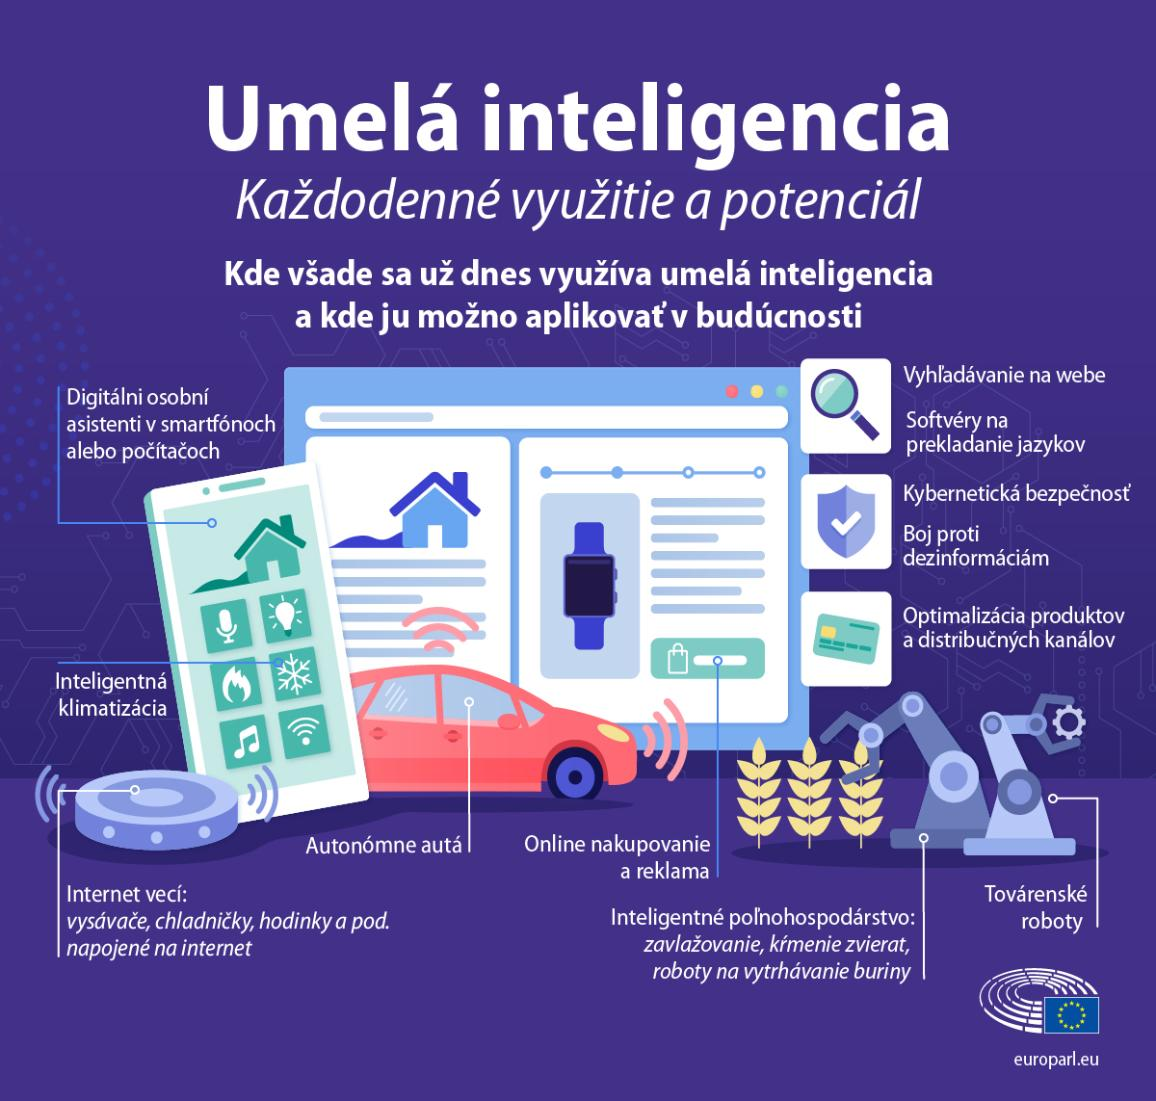
\includegraphics[width=.9\textwidth]{figures/vyuzitie-a-potencia-ai.png}
    \caption{Využitie a potencial AI}
\end{figure}


Na obrázku č. 1.7 môžeme vidieť aké sú možnosti uplatnenia AI. Medzi možnosti uplatnenia AI patrí: inteligentná klimatizácia, digitálni osobní asistenti v smartfónoch alebo počítačoch, internet vecí - vysávače, chladničky, hodinky, autonómne automobily, online nakupovanie a reklama, vyhľadávanie na webe, softvéry na prekladanie jazykov, kybernetická bezpečnosť, boj proti dezinformáciám, optimalizácia produktov a distribučných kanálov, továrenské roboty, inteligentné poľnohospodárstvo - zavlažovanie, kŕmenie zvierat, roboty na vytrhávanie buriny, a iné.  Môžeme vidieť, že možnosti uplatnenia AI nástrojov sú širokospektrálne.\cite{eu_parliament_ai}
\par Niektoré technológie založené na AI už existujú viac rokov. Avšak v posledných rokoch vďaka pokrokom vo výpočtovej technike, dostupnosti enormného množstva dát a novým algoritmom sa vyvíjajú modernejšie AI online nástroje s inovatívnymi riešeniami. \cite{eu_parliament_ai}
\par Príchod moderných AI online nástrojov zmenil výrazne postoj ľudí alebo podnikov pozitívnym smerom v tejto problematike. Moderné AI online nástroje sú považované v súčasnosti skôr za príležitosť. Aj odborníci radia, aby aplikácia AI online nástrojov bola nielen obrovskou príležitosťou ale hlavne konkurenčnou výhodou a mať otvorený prístup k novým zmenám. \cite{removcikova_ai}  Avšak musia sa odstrániť rôzne bariéry, ktoré implementovaniu moderných AI online nástrojov bránia ako napríklad:

\begin{itemize}
    \item používateľ AI online nástrojov nemá prehľad o ich algoritmoch a procesoch
    \item k moderným AI nástrojom zvykneme mať tendenciu zaujatosti
    \item učenie AI nástrojov si vyžaduje ešte čas, aby boli aj výkonnejšie, atď... 
\end{itemize} 


Hlavným prínosom využívania AI online nástrojov je vyššia efektívnosť, čo predstavuje úsporu času a ľudských zdrojov.  AI online nástroje zvyšujú rýchlosť aj v generovaní požadovaných výstupov. Moderné AI online nástroje vynikajú nielen rýchlosťou ale i vylepšenou presnosťou generovania výstupov, čo umožňuje podnikom sústrediť sa na dôležitejšie core činnosti. \cite{deng2022} V súčasnosti ide už o výkonnejšie modely AI nástrojov so získavaním výstupov v reálnom čase a so znižovaním rôznych nákladov pre zefektívnenie podnikových procesom, a iné.
\par Dospeli sme nielen k pozitívam využívania AI online nástrojov ale i k výzvam respektíve k obmedzeniam, ktorými sú AI online nástroje stále sprevádzané. V diplomovej práci by sme chceli vybrať niektoré z dostupných AI online nástroje na trhu a zanalyzovať ich. Pretože AI online nástroje na trhu sú vo všeobecnosti sľubnou technológiou do budúcnosti.



% ------------------------------ Súčasné trendy AI online nástrojovv -------------------------------

\subsection{Súčasné trendy AI online nástrojov}

V súčasnosti je už na trhu veľké množstvo AI online nástrojov. Podľa najväčšej českej databázy AI nástrojov celkový počet AI nástrojov je až 2 691. \cite{ejaj} S najväčším počtom AI online nástrojov sú tieto kategórie:
\begin{itemize}
    \item produktivita - ChatGPT, Durable, Cody, Casper AI
    \item životný asistent - Roamaround, Where TO, ProductBot
    \item všeobecné písanie - GPT3 Playground, Analogenie
    \item vývojárske nástroje - Pinecone, Datature, One AI
    \item asistent pre vzdelávanie - WolframAlpha, Wisdolia
    \item zábavné nástroje - Scribble Diffusion, The GPT Who Lived, Booom.ai
    \item copywriting - Jasper, Rytr, Yaara
    \item generátor obrázkov - Stable Diffusion, Lucidpic, Pebblely
    \item zákaznícka podpora - Second Nature AI, TheLoops, Yuma
    \item dizajnový asistent - Galileo, Flair AI, Autodraw
    \item predaj - Second Nature AI, Octane AI
    \item e-mail asistent - HoppyCopy, Rytr, Superflows
    \item asistent pre sociálne média - Piggy To, Predict AI, Morise.ai
    \item SEO - LongShot, Moonbeam, SheetAI.app
    \item výskum/vývoj - Laion, Arxiv Feed
    \item programovanie a vývoj - Codeium, Replit, Lookup, SourceAI, Google Bard, Code GPT, Maverick, Hey, GitHub copilot, GPT95, GitFluence, Safurai, Cron AI, Amazon CodeWhisperer, Spellbox, Xata, Codium AI, Code Snippets AI,...
    \item low-code/no-code a ďalšie iné kategórie - ChatGPT Website Builder, Browse AI, Block Survey.
\end{itemize}

Umelá inteligencia dokáže významne uľahčiť prácu copywriterom, grafickým dizajnérom a podnikom.  Okrem týchto najbežnejších využitiach AI online nástrojov v každodennom živote je nápomocná aj pri programovaní. \cite{brabencova_programatori_2023}
\par V diplomovej práci práve zvolíme tie AI online nástroje, ktoré súvisia práve s programovaním. Pretože programovanie značne uľahčuje programátorom prácu prostredníctvom AI online nástrojov určených na vytváranie kódov.



% --------------------------- Úloha AI online nástrojov v programovaní -----------------------------


\section{Úloha AI online nástrojov v programovaní}

AI sa stáva čoraz dôležitejším nástrojom v rôznych odvetviach a to sa týka aj programovania.  Zjednodušenie pre programátorov je hlavne automatizácia.  Práve prostredníctvom AI online nástrojov je možné zrýchliť a zefektívniť kód.  Dokonca niektoré moderné AI online nástroje v súčasnosti už dokážu analyzovať dátové štruktúry a navrhnúť optimálný model databázy, čo zjednodušuje programátorom dosť prácu a predchádzajú tak vznikajúcim chybám. \cite{brabencova_programatori_2023}
\par Medzi ďalší spôsob, ktorý uľahčuje prácu programátorov prostredníctvom využívania AI online nástrojov, patrí testovanie a ladenie kódu. AI online nástroje dokonca môžu testovať aplikácie, čím sa zvýši kvalita softvéru a programátori sa môžu venovať iným novo-vytvárajúcim funkciám a zlepšovaniu aplikácií. \cite{brabencova_programatori_2023}
\par Ako uviedla Brabencová (2023), programátorov budeme stále potrebovať v súbehu prichádzajúcich nových výziev v oblasti AI. Práca programátorov vôbec nevymizne. Práveže zručnosti programátorov a ich rozvoj bude kľúčový v budúcnosti. Zautomatizujú sa len rutinné činnosti a zvýši sa efektivita vývoja softvéru. \cite{brabencova_programatori_2023}
\par Dominik (2023) potvrdil, že uľahčenie programovania už môžeme vidieť vďaka súčasným AI online nástrojom ako je napríklad chatbot ChatGPT, pretože dokáže generovať jednoduchšie kódy v programovacích jazykoch.  \cite{dominik_ai_programovanie}
\par S rastúcom rozmanitosťou programovacích jazykov rastie aj potreba prekladať programy z jedného programovacieho jazyka do iného programovacieho jazyka.  Ide o tzv. preklad programovacích jazykov, čo nám zefektívňuje nielen prácu ale môžeme opätovne použiť existujúci kód, hlavne ak sa dá preklad zautomatizovať.  Program, ktorý bol vyvinutý v jednom programovacom jazyku je možné preložiť do iného programovacieho jazyka a zároveň zdrojový kód v jednom programovacom jazyku je možné prekonvertovať do iného jazyka.\cite{kj_preklad_jazyka}
\par Naším zameraním v diplomovej práci bude zhodnotenie prekladu programovacích jazykov v AI online nástrojov ako hlavnej problematiky témy Využívania AI online nástrojov pri preklade programovacích jazykov. Preskúmať do akej miery dokážu niektoré AI online nástroje prekladať programovacie jazyky. Pretože AI online nástroje, ktoré sú určené na preklad programovacích jazykov, môžu byť nápomocné pri zistení nedostatkov a urýchleniu vývoja a iných faktorov s cieľom efektívnej implementácie v AI nástrojoch.



% ------------------ Uľahčovanie programovania prostredníctvom AI na základe faktorov --------------

\subsection{Uľahčovanie programovania prostredníctvom AI na základe faktorov}

Programovanie prechádza výrazným pokrokom s cieľom uľahčiť a zdokonaliť prácu programátora. Prostredníctvom vývoja AI v programovaní sa otvárajú nové možnosti v AI online nástrojoch, pri ktorých pozorujeme ich vlastné kombinácie vlastností. Medzi hlavné vlastnosti programu (ukazovatele kvality) zaraďujeme:

\begin{itemize}
    \item korektnosť (správnosť)
    \item spoľahlivosť (robustnosť)
    \item efektívnosť
    \item rýchlosť
    \item rozšíriteľnosť
    \item kompatibilita
    \item dostupnosť
    \item modifikovateľnosť
    \item používateľsky prívetivé spracovanie (user friendly) a podobne. 
\end{itemize}

Tieto faktory sú pozorované programátormi pri preklade programovacích jazykov a stávajú sa hlavnou podporou vo vývoji AI online nástrojov a využívania pokročilých technológií pre uľahčenie programovania.
\par V diplomovej práci ďalej chceme zamerať pozornosť na faktory, akými sú presnosť prekladu programovacích jazykov, podpora programovacích jazykov, dopad na výkon a riešenie prekladu špecifických jazykových konštrukcií, ktoré iné jazyky priamo nepodporujú. To splníme vlastným experimentovaním, na základe čoho vyvodíme závery.



% --------------------------------- Budúcnosť AI v programovaní -------------------------------------------

\subsection{Budúcnosť AI v programovaní}

V najbližších rokoch AI sa bude vyznačovať väčšou spoľahlivosťou spájať jednotlivé sub-kódy pre konkrétne funkcionality do plne funkčného komplexného kódu.  Aj napriek tomu, že programátori budú stále potrební, môžu podniky znížiť stav ľudských zdrojov vďaka AI. Pretože AI, ako sme spomínali, dokáže zjednodušiť prácu programátorov a ich niektorých opakujúcich sa činností a tým pádom môže nastať pokles až o 25 \% programátorov. \cite{dominik_ai_programovanie}
\par Tiež v blízkej budúcnosti sa môžeme dočkať kompletných SaaS programovacích nástrojov, ktoré budú generovať finálne softvérové produkty len na základe textových príkazov v chate.  Čiže nebudeme musieť napísať ani kúsok klasického kódu. Príkladom takéhoto programovania bez IDE a kódov je príklad AI, ktorá na základe myšlienky vytvorí kompletnú webstránku v súlade s pravidlami psychológie predaja a najnovšími trendami. \cite{dominik_ai_programovanie}
\par Oveľa neskôr na základe predošlých prognóz budúcnosti v oblasti AI bude možné automaticky vytvorené webstránky alebo aplikácie automaticky optimalizovať, automaticky upravovať obsah na webe vďaka budúcej AI.  To znamená, že nebude potrebný žiadny ľudský zásah do svojho webu alebo aplikácie. \cite{dominik_ai_programovanie}
\par Na základe zhromaždenia budúcich prognóz v oblasti AI a programovania môžeme tvrdiť, že vývoj AI už dnes zaznamenal rýchly pokrok. Preto táto diplomová práca by sa mala venovať aj súčasným limitáciám AI online nástrojov v programovaní pri preklade programovacích jazykov. \cite{dominik_ai_programovanie}



 
\chapter{Analýza a rozbor AI online nástrojov}
\section{Chat GPT}
\subsection{Chat GPT 3.5}
\subsection{Chat GPT 4.0 - spoplatnená verzia}
\section{Google Bard}
\section{Code Convert}
\section{AI Code Convertor}

\chapter{Analýza programovacích jazykov}
\section{Kritéria výberu programovacieho jazyka}
\section{Programovacie jazyky}
\subsection{Java}
\subsection{C++}
\subsection{Python}
\subsection{Assembler}



% !TEX root = ../thesis.tex

\chapter{Syntetická časť}
\label{methodology}

Syntetická časť opisuje metódy použité na syntézu riešenia a opisuje syntézu samotného riešenia (zvyčajne je to návrh/implementácia softvérového resp. hardvérového riešenia), pričom sa opiera o~závery analytickej časti práce. Začína od toho, ako sa bude riešenie používať: najdôležitejšie scenáre používania a používateľské rozhranie, ktoré bude tieto scenáre efektívne podporovať. Až potom je na rade vnútorná architektúra alebo použité technológie. Syntetická časť tvorí zvyčajne ½ jadra práce.

Syntetickú časť práce vhodne rozdeľte do kapitol a pomenujte ich podľa toho, čomu sú venované.

% !TEX root = ../thesis.tex

\chapter{Vyhodnotenie}
\label{evaluation}

Vyhodnocovacia časť je kľúčovou časťou záverečnej práce. Tato časť obsahuje vyhodnotenie navrhnutého (vytvoreného) riešenia. Uprednostňované je objektívne vyhodnotenie výsledkov práce, ktoré sa opiera o~meranie a štatistické metódy, prípadne matematické dôkazy. V~prípade nameraných hodnôt musí autor opísať metódu merania, priebeh merania, výsledky a interpretáciu výsledkov v~kontexte riešeného problému a stanovených cieľov. Na základe vyhodnotenia riešenia autor opíše prínosy svojej práce. Vyhodnocovacia časť tvorí zvyčajne ¼ jadra práce.

% !TEX root = ../thesis.tex

\chapter{Záver}
\label{summary}

Záver práce obsahuje zhrnutie výsledkov práce s~jasným opisom prínosov a pôvodných (vlastných) výsledkov autora a vyhodnotenie splnenia stanovených cieľov. Je to stručné zhrnutie informácií uvedených v~záverečnej práci. Záver by nemal obsahovať nové informácie.

V~závere by mal tiež autor poukázať na prípadné otvorené otázky, ktoré sú nad rámec rozsahu práce a mal by odporučiť ďalšie aktivity na pokračovanie pri riešení problému. Rozsah záveru je minimálne 1 celá strana.


% good linebraking of bibtex url
\setcounter{biburllcpenalty}{7000}
\setcounter{biburlucpenalty}{8000}

%% The bibliography
\printbibliography[heading=bibintoc]

\label{theend} % the last page of the thesis

% List of acronyms
\printglossary[type=\acronymtype,title={\acrlistname}]

% Glossaries
\printglossary

%% Appendix
% !TEX root = ../thesis.tex

\chapter*{\appendixlistname}
\addcontentsline{toc}{chapter}{\appendixlistname}

\begin{description}
	\item[\appendixname{} A] Karel Language Reference
    \item[\appendixname{} B] CD médium -- záverečná práca v~elektronickej podobe,
    \item[\appendixname{} C] Používateľská príručka
    \item[\appendixname{} D] Systémová príručka
\end{description}

\appendix
\renewcommand\chaptername{\appendixname}
\section{\textbf{Použitá literatúra - zistiť ako to sfromatovať a správne zaradiť }}

\begin{itemize}
    \item Benavides, Eduardo \& Fuertes, Walter \& Sanchez-Gordon, Sandra \& Sanchez, Manuel. (2020). Classification of Phishing Attack Solutions by Employing Deep Learning Techniques: A Systematic Literature Review. 10.1007/978-981-13-9155-2\_5.
  
    \item EMANS. Umelá inteligencia začína prekopávať fungovanie domácich firiem ?  [online]. Aktualizované  22-07-2019, cit. [19-01-2024].  
    \par https://www.anasoft.com/emans/sk/home/Novinky-blog/blog/ \par Umela-inteligencia-zmeni-priemysel-a-logistiku
   
    \item ENHOLM, Ida Merete, et al. Artificial intelligence and business value: A literature review. Information Systems Frontiers, 2022, 24.5: 1709-1734.
   
    \item ENHOLM, Ida Merete, et al. Artificial intelligence and business value: A literature review. Information Systems Frontiers, 2022, 24.5: 1709-1734.
    \item GLÓS, PRÁCE KRISTIÁN. HLBOKÉ UČENIE AI V HERNÝCH PROSTREDIACH.
    \item Hlásny, M. (2023). Vplyv digitalizácie na pracovný proces. Digitálne kompetencie žiakov a učiteľov v kontexte informatizácie a digitalizácie školstva.
    \item Chernyak, A., Z. Počítačové videnie je budúcnosťou automatizácie testovania softvéru - história minulosti, súčasnosti a budúcnosti [online]. Aktualizované  09-12-2022, cit. [19-01-2024]. https://www.zaptest.com/sk/pocitacove-videnie-je-buducnostou-automatizacie-testovania-softveru-historia-minulosti-sucasnosti-a-buducnosti
    \item Kanade, V. (2022). What Is Artificial Intelligence (AI) Definition, Types, Goals, Challenges and Trends in 2022 [online]. Upload 14-03-2022, cit. [19-01-2024]. https://www.spiceworks.com/tech/artificial-intelligence/articles/what-is-ai/
    \item Kolbjørnsrud, V., Amico, R., \& Thomas, R. J. (2017). Partnering with AI: how organizations can win over skeptical managers. Strategy \& Leadership, 45(1), 37–43
    \item KORNIENKO, Alla A., et al. Knowledge in artificial intelligence systems: searching the strategies for application. Procedia-Social and Behavioral Sciences, 2015, 166: 589-594.
    \item Krajči, M. (2020).Využití neurónových sítí a uměle inteligence v marketingu. Brno: AMBIS.
    \item Lee, J., Suh, T., Roy, D.,\& Baucus, M. (2019). Emerging technology and business model innovation: the case of artificial intelligence. Journal of Open Innovation: Technology, Market, and Complexity, 5(3), 44
    \item Makarius, E. E., Mukherjee, D., Fox, J. D.\& Fox, A. K. (2020). Rising with the machines: A sociotechnical framework for bringing artifi- cial intelligence into the organization. Journal of Business Research, 120, 262–273
    \item Mikalef, P., Pappas, I. O., Krogstie, J., \& Giannakos, M. (2018). Big data analytics capabilities: a systematic literature review and research agenda. Information Systems and e-Business Management, 16(3), 547–578
    \item Nelson, D. Čo je to NLP (spracovanie prirodzeného jazyka)? [online]. Aktualizované  09-12-2022, cit. [19-01-2024]. \par https://www.unite.ai/sk/čo-je-spracovanie-prirodzeného-jazyka/
    \item SCALER. Top 10 Characteristics of Artificial Intelligence [online]. Aktualizované  08-01-2024, cit. [19-01-2024]. \par https://www.interviewbit.com/blog/characteristics-of-artificial-intelligence/
    \item Schmidt, R., Zimmermann, A., Moehring, M., \& Keller, B. (2020). Value creation in connectionist artificial intelligence–A research agenda
    \item ŠTALMACHOVÁ, Katarína; STRENITZEROVÁ, Mariana. Umelá inteligencia, strojové učenie a trh práce. 2020.
    \item Tencent Research Institute, CAICT, Tencent AI Lab, Tencent open platform (2021). Artificial Intelligence: A National Strategic Initiative. Beijing: Palgrave Macmillan. ISBN: 978-981-15-6547-2.
    \item Tököly, R. Táto technológia otvorí robotom úplne nové možnosti, umelá inteligencia ich posunie míľovými krokmi [online]. Aktualizované  25-05-2023, cit. [19-01-2024]. https://fontech.startitup.sk/tato-technologia-otvori-robotom-uplne-nove-moznosti-umela-inteligencia-ich-posunie-milovymi-kromi/
    \item ToolsForHumans. AI Statistics And Trends For 2023 [online]. Updated 04-08-2023, cit. [19-01-2024]. \par https://assets-global.website-files.com/63a3450e7d71b8e0c27ad3b6/6\par 4c226014a9b193611c5a2b9\_Artificial- \par Intelligence-Market-Size-2021-to-2030-1600x947.webp
    \item Vrba, F. (2019). Od ľudského vedomia k umelej inteligencii [online]. Cit. [19-01-2024]. Brno: Masarykova univerzita. \par https://www.google.com/url?sa=t\&rct=j\&q=\&esrc=s\&source= 
\par web\&cd=\&ved=2ahUKEwi3uMr3rOyDAxV7i \par \_0HHZmxDvwQFnoECBEQAQ\&url=https\%3A\ 
  \par \%2F\%2Fis.muni.cz\%2Fth\%2Fcsmt4\%2F43 \par 3764\_bakalarska\_praca \par \_Archive.pdf\&usg=AOvVaw00Ea3j7-jXnIvJH0axIK-C\&opi=89978449
    \item Wamba-Taguimdje, S. L., Wamba, S. F., Kamdjoug, J. R. K., \& Wanko, C. E. T. (2020). Influence of artificial intelligence (AI) on firm performance: the business value of AI-based transformation pro- jects. Business Process Management Journal, 26(7), 1893–1924. https://doi.org/10.1108/BPMJ-10-2019-0411
    \item Wang, H., Huang, J., \& Zhang, Z. (2019). The impact of deep learning on organizational agility. In proceedings of the 40th International Conference on Information Systems (ICIS), Munich, Germany
    \item HOLMSTRÖM, Jonny. From AI to digital transformation: The AI readiness framework. Business Horizons, 2022, 65.3: 329-339.
    \item EMEA. What Is a Digital Transformation Framework? [online]. Aktualizované  28-04-2021, cit. [19-01-2024]. https://www.salesforce.com/eu/blog/what-is-digital-transformation-framework/
    \item Aspecta. Trendy digitálnej transformácie roku 2021 [online]. Cit. [19-01-2024]. https://aspecta.sk/trendy-digitalnej-transformacie-roku-2021/
    \item Európsky parlament. Umelá inteligencia: definícia a využitie [online]. Aktualizované  21-06-2023, cit. [19-01-2024]. \par https://www.europarl.europa.eu/news/sk/headlines/society/ \par 20200827STO85804/umela-inteligencia-definicia-a-vyuzitie
    \item Removčíková, L. Umelá inteligencia a jej využitie (nielen) vo firmách [online]. Aktualizované  21-06-2023, cit. [19-01-2024]. \par https://www.podnikajte.sk/technologie/umela-inteligencia-a-jej-vyuzitie
    \item VENKATESH, Viswanath. Adoption and use of AI tools: a research agenda grounded in UTAUT. Annals of Operations Research, 2022, 1-12.
    \item DENG, Jianyang; LIN, Yijia. The benefits and challenges of ChatGPT: An overview. Frontiers in Computing and Intelligent Systems, 2022, 2.2: 81-83.
    \item Brabencová, P. Budúcnosť programátorov a umelej inteligencie [online]. Aktualizované  18-10-2023, cit. [19-01-2024]. https://itide.sk/blog/buducnost-programatorov-a-umelej-inteligencie
    \item Dominik. Umelá inteligencia a programovanie: Pozrite sa, ako Vám uľahčí život! [online]. Aktualizované  25-03-2023, cit. [19-01-2024].\par https://monkeymedia.sk/umela-inteligencia-a-programovanie-pozrite-sa-ako-vam-ulahci-zivot/
    \item Jurinová, J. Algoritmizácia a základy štruktúrovaného programovania v jazyku C. 1.vydanie. Trnava: Univerzita sv. Cyrila a Metoda, 2020. ISBN: 978-80-8105-859-2.
    \item Paschen, J., Kietzmann, J., \& Kietzmann, T. C. (2019). Artificial intelligence (AI) and its implications for market knowledge in B2B marketing. Journal of Business and Industrial Mar- keting, 34(7), 1410e1419.
    \item PASCHEN, Ulrich; PITT, Christine; KIETZMANN, Jan. Artificial intelligence: Building blocks and an innovation typology. Business Horizons, 2020, 63.2: 147-155.
    \item K\&J. Preklad programovacieho jazyka [online]. Aktualizované  11-08-2022, cit. [19-01-2024]. https://www.kjtranslations.sk/blog/preklad-programovacieho-jazyka/
    \item Ejaj. Největší česká databáze AI nástrojů [online]. Cit. [19-01-2024]. https://ejaj.cz/
    \item Ayça, E. Definitions of AI [online]. Aktualizované  24-11-2019, cit. [19-01-2024]. https://elizaycayilmaz.medium.com/definitions-of-ai-5efb8989db09
    \item SAP. Čo je to umelá inteligencia? [online]. Cit. [19-01-2024]. \par https://www.sap.com/sk/products/artificial-intelligence/what-is-artificial-intelligence.html
\end{itemize}

% zivotopis autora
%\curriculumvitae\protect
%Táto časť\/ je nepovinná. Autor tu môže uviesť\/ svoje biografické
%údaje, údaje o~záujmoch, účasti na~projektoch, účasti na~súťažiach,
%získané ocenenia, zahraničné pobyty na~praxi, domácu prax, publikácie
%a~pod.

\end{document}